\documentclass{report}
% package para el simbolo dotminus
\usepackage{amsmath}

% macro para dotminus
\makeatletter
\newcommand{\dotminus}{\mathbin{\text{\@dotminus}}}
\newcommand{\@dotminus}{%
  \ooalign{\hidewidth\raise1ex\hbox{.}\hidewidth\cr$\m@th-$\cr}%
}
\makeatother


%%%%%%%%%%%%%%%%%%%%%%%%%%%%%%%%%
% PACKAGE IMPORTS
%%%%%%%%%%%%%%%%%%%%%%%%%%%%%%%%%


\usepackage[tmargin=2cm,rmargin=1in,lmargin=1in,margin=0.85in,bmargin=2cm,footskip=.2in]{geometry}
\usepackage{amsmath,amsfonts,amsthm,amssymb,mathtools}
\usepackage[varbb]{newpxmath}
\usepackage{xfrac}
\usepackage[makeroom]{cancel}
\usepackage{mathtools}
\usepackage{bookmark}
\usepackage{enumitem}
\usepackage{hyperref,theoremref}
\hypersetup{
	pdftitle={Assignment},
	colorlinks=true, linkcolor=doc!90,
	bookmarksnumbered=true,
	bookmarksopen=true
}
\usepackage[most,many,breakable]{tcolorbox}
\usepackage{xcolor}
\usepackage{varwidth}
\usepackage{varwidth}
\usepackage{etoolbox}
%\usepackage{authblk}
\usepackage{nameref}
\usepackage{multicol,array}
\usepackage{tikz-cd}
\usepackage[ruled,vlined,linesnumbered]{algorithm2e}
\usepackage{comment} % enables the use of multi-line comments (\ifx \fi) 
\usepackage{import}
\usepackage{xifthen}
\usepackage{pdfpages}
\usepackage{transparent}

\newcommand\mycommfont[1]{\footnotesize\ttfamily\textcolor{blue}{#1}}
\SetCommentSty{mycommfont}
\newcommand{\incfig}[1]{%
    \def\svgwidth{\columnwidth}
    \import{./figures/}{#1.pdf_tex}
}

\usepackage{tikzsymbols}
\renewcommand\qedsymbol{$\Laughey$}


%\usepackage{import}
%\usepackage{xifthen}
%\usepackage{pdfpages}
%\usepackage{transparent}


%%%%%%%%%%%%%%%%%%%%%%%%%%%%%%
% SELF MADE COLORS
%%%%%%%%%%%%%%%%%%%%%%%%%%%%%%



\definecolor{myg}{RGB}{56, 140, 70}
\definecolor{myb}{RGB}{45, 111, 177}
\definecolor{myr}{RGB}{199, 68, 64}
\definecolor{mytheorembg}{HTML}{F2F2F9}
\definecolor{mytheoremfr}{HTML}{00007B}
\definecolor{mylenmabg}{HTML}{FFFAF8}
\definecolor{mylenmafr}{HTML}{983b0f}
\definecolor{mypropbg}{HTML}{f2fbfc}
\definecolor{mypropfr}{HTML}{191971}
\definecolor{myexamplebg}{HTML}{F2FBF8}
\definecolor{myexamplefr}{HTML}{88D6D1}
\definecolor{myexampleti}{HTML}{2A7F7F}
\definecolor{mydefinitbg}{HTML}{E5E5FF}
\definecolor{mydefinitfr}{HTML}{3F3FA3}
\definecolor{notesgreen}{RGB}{0,162,0}
\definecolor{myp}{RGB}{197, 92, 212}
\definecolor{mygr}{HTML}{2C3338}
\definecolor{myred}{RGB}{127,0,0}
\definecolor{myyellow}{RGB}{169,121,69}
\definecolor{myexercisebg}{HTML}{F2FBF8}
\definecolor{myexercisefg}{HTML}{88D6D1}


%%%%%%%%%%%%%%%%%%%%%%%%%%%%
% TCOLORBOX SETUPS
%%%%%%%%%%%%%%%%%%%%%%%%%%%%

\setlength{\parindent}{1cm}
%================================
% THEOREM BOX
%================================

\tcbuselibrary{theorems,skins,hooks}
\newtcbtheorem[number within=section]{Theorem}{Theorem}
{%
	enhanced,
	breakable,
	colback = mytheorembg,
	frame hidden,
	boxrule = 0sp,
	borderline west = {2pt}{0pt}{mytheoremfr},
	sharp corners,
	detach title,
	before upper = \tcbtitle\par\smallskip,
	coltitle = mytheoremfr,
	fonttitle = \bfseries\sffamily,
	description font = \mdseries,
	separator sign none,
	segmentation style={solid, mytheoremfr},
}
{th}

\tcbuselibrary{theorems,skins,hooks}
\newtcbtheorem[number within=chapter]{theorem}{Theorem}
{%
	enhanced,
	breakable,
	colback = mytheorembg,
	frame hidden,
	boxrule = 0sp,
	borderline west = {2pt}{0pt}{mytheoremfr},
	sharp corners,
	detach title,
	before upper = \tcbtitle\par\smallskip,
	coltitle = mytheoremfr,
	fonttitle = \bfseries\sffamily,
	description font = \mdseries,
	separator sign none,
	segmentation style={solid, mytheoremfr},
}
{th}


\tcbuselibrary{theorems,skins,hooks}
\newtcolorbox{Theoremcon}
{%
	enhanced
	,breakable
	,colback = mytheorembg
	,frame hidden
	,boxrule = 0sp
	,borderline west = {2pt}{0pt}{mytheoremfr}
	,sharp corners
	,description font = \mdseries
	,separator sign none
}

%================================
% Corollery
%================================
\tcbuselibrary{theorems,skins,hooks}
\newtcbtheorem[number within=section]{Corollary}{Corollary}
{%
	enhanced
	,breakable
	,colback = myp!10
	,frame hidden
	,boxrule = 0sp
	,borderline west = {2pt}{0pt}{myp!85!black}
	,sharp corners
	,detach title
	,before upper = \tcbtitle\par\smallskip
	,coltitle = myp!85!black
	,fonttitle = \bfseries\sffamily
	,description font = \mdseries
	,separator sign none
	,segmentation style={solid, myp!85!black}
}
{th}
\tcbuselibrary{theorems,skins,hooks}
\newtcbtheorem[number within=chapter]{corollary}{Corollary}
{%
	enhanced
	,breakable
	,colback = myp!10
	,frame hidden
	,boxrule = 0sp
	,borderline west = {2pt}{0pt}{myp!85!black}
	,sharp corners
	,detach title
	,before upper = \tcbtitle\par\smallskip
	,coltitle = myp!85!black
	,fonttitle = \bfseries\sffamily
	,description font = \mdseries
	,separator sign none
	,segmentation style={solid, myp!85!black}
}
{th}


%================================
% LENMA
%================================

\tcbuselibrary{theorems,skins,hooks}
\newtcbtheorem[number within=section]{Lenma}{Lenma}
{%
	enhanced,
	breakable,
	colback = mylenmabg,
	frame hidden,
	boxrule = 0sp,
	borderline west = {2pt}{0pt}{mylenmafr},
	sharp corners,
	detach title,
	before upper = \tcbtitle\par\smallskip,
	coltitle = mylenmafr,
	fonttitle = \bfseries\sffamily,
	description font = \mdseries,
	separator sign none,
	segmentation style={solid, mylenmafr},
}
{th}

\tcbuselibrary{theorems,skins,hooks}
\newtcbtheorem[number within=chapter]{lenma}{Lenma}
{%
	enhanced,
	breakable,
	colback = mylenmabg,
	frame hidden,
	boxrule = 0sp,
	borderline west = {2pt}{0pt}{mylenmafr},
	sharp corners,
	detach title,
	before upper = \tcbtitle\par\smallskip,
	coltitle = mylenmafr,
	fonttitle = \bfseries\sffamily,
	description font = \mdseries,
	separator sign none,
	segmentation style={solid, mylenmafr},
}
{th}


%================================
% PROPOSITION
%================================

\tcbuselibrary{theorems,skins,hooks}
\newtcbtheorem[number within=section]{Prop}{Proposition}
{%
	enhanced,
	breakable,
	colback = mypropbg,
	frame hidden,
	boxrule = 0sp,
	borderline west = {2pt}{0pt}{mypropfr},
	sharp corners,
	detach title,
	before upper = \tcbtitle\par\smallskip,
	coltitle = mypropfr,
	fonttitle = \bfseries\sffamily,
	description font = \mdseries,
	separator sign none,
	segmentation style={solid, mypropfr},
}
{th}

\tcbuselibrary{theorems,skins,hooks}
\newtcbtheorem[number within=chapter]{prop}{Proposition}
{%
	enhanced,
	breakable,
	colback = mypropbg,
	frame hidden,
	boxrule = 0sp,
	borderline west = {2pt}{0pt}{mypropfr},
	sharp corners,
	detach title,
	before upper = \tcbtitle\par\smallskip,
	coltitle = mypropfr,
	fonttitle = \bfseries\sffamily,
	description font = \mdseries,
	separator sign none,
	segmentation style={solid, mypropfr},
}
{th}


%================================
% CLAIM
%================================

\tcbuselibrary{theorems,skins,hooks}
\newtcbtheorem[number within=section]{claim}{Claim}
{%
	enhanced
	,breakable
	,colback = myg!10
	,frame hidden
	,boxrule = 0sp
	,borderline west = {2pt}{0pt}{myg}
	,sharp corners
	,detach title
	,before upper = \tcbtitle\par\smallskip
	,coltitle = myg!85!black
	,fonttitle = \bfseries\sffamily
	,description font = \mdseries
	,separator sign none
	,segmentation style={solid, myg!85!black}
}
{th}



%================================
% Exercise
%================================

\tcbuselibrary{theorems,skins,hooks}
\newtcbtheorem[number within=section]{Exercise}{Exercise}
{%
	enhanced,
	breakable,
	colback = myexercisebg,
	frame hidden,
	boxrule = 0sp,
	borderline west = {2pt}{0pt}{myexercisefg},
	sharp corners,
	detach title,
	before upper = \tcbtitle\par\smallskip,
	coltitle = myexercisefg,
	fonttitle = \bfseries\sffamily,
	description font = \mdseries,
	separator sign none,
	segmentation style={solid, myexercisefg},
}
{th}

\tcbuselibrary{theorems,skins,hooks}
\newtcbtheorem[number within=chapter]{exercise}{Exercise}
{%
	enhanced,
	breakable,
	colback = myexercisebg,
	frame hidden,
	boxrule = 0sp,
	borderline west = {2pt}{0pt}{myexercisefg},
	sharp corners,
	detach title,
	before upper = \tcbtitle\par\smallskip,
	coltitle = myexercisefg,
	fonttitle = \bfseries\sffamily,
	description font = \mdseries,
	separator sign none,
	segmentation style={solid, myexercisefg},
}
{th}

%================================
% EXAMPLE BOX
%================================

\newtcbtheorem[number within=section]{Example}{Example}
{%
	colback = myexamplebg
	,breakable
	,colframe = myexamplefr
	,coltitle = myexampleti
	,boxrule = 1pt
	,sharp corners
	,detach title
	,before upper=\tcbtitle\par\smallskip
	,fonttitle = \bfseries
	,description font = \mdseries
	,separator sign none
	,description delimiters parenthesis
}
{ex}

\newtcbtheorem[number within=chapter]{example}{Example}
{%
	colback = myexamplebg
	,breakable
	,colframe = myexamplefr
	,coltitle = myexampleti
	,boxrule = 1pt
	,sharp corners
	,detach title
	,before upper=\tcbtitle\par\smallskip
	,fonttitle = \bfseries
	,description font = \mdseries
	,separator sign none
	,description delimiters parenthesis
}
{ex}

%================================
% DEFINITION BOX
%================================

\newtcbtheorem[number within=section]{Definition}{Definition}{enhanced,
	before skip=2mm,after skip=2mm, colback=red!5,colframe=red!80!black,boxrule=0.5mm,
	attach boxed title to top left={xshift=1cm,yshift*=1mm-\tcboxedtitleheight}, varwidth boxed title*=-3cm,
	boxed title style={frame code={
					\path[fill=tcbcolback]
					([yshift=-1mm,xshift=-1mm]frame.north west)
					arc[start angle=0,end angle=180,radius=1mm]
					([yshift=-1mm,xshift=1mm]frame.north east)
					arc[start angle=180,end angle=0,radius=1mm];
					\path[left color=tcbcolback!60!black,right color=tcbcolback!60!black,
						middle color=tcbcolback!80!black]
					([xshift=-2mm]frame.north west) -- ([xshift=2mm]frame.north east)
					[rounded corners=1mm]-- ([xshift=1mm,yshift=-1mm]frame.north east)
					-- (frame.south east) -- (frame.south west)
					-- ([xshift=-1mm,yshift=-1mm]frame.north west)
					[sharp corners]-- cycle;
				},interior engine=empty,
		},
	fonttitle=\bfseries,
	title={#2},#1}{def}
\newtcbtheorem[number within=chapter]{definition}{Definition}{enhanced,
	before skip=2mm,after skip=2mm, colback=red!5,colframe=red!80!black,boxrule=0.5mm,
	attach boxed title to top left={xshift=1cm,yshift*=1mm-\tcboxedtitleheight}, varwidth boxed title*=-3cm,
	boxed title style={frame code={
					\path[fill=tcbcolback]
					([yshift=-1mm,xshift=-1mm]frame.north west)
					arc[start angle=0,end angle=180,radius=1mm]
					([yshift=-1mm,xshift=1mm]frame.north east)
					arc[start angle=180,end angle=0,radius=1mm];
					\path[left color=tcbcolback!60!black,right color=tcbcolback!60!black,
						middle color=tcbcolback!80!black]
					([xshift=-2mm]frame.north west) -- ([xshift=2mm]frame.north east)
					[rounded corners=1mm]-- ([xshift=1mm,yshift=-1mm]frame.north east)
					-- (frame.south east) -- (frame.south west)
					-- ([xshift=-1mm,yshift=-1mm]frame.north west)
					[sharp corners]-- cycle;
				},interior engine=empty,
		},
	fonttitle=\bfseries,
	title={#2},#1}{def}



%================================
% Solution BOX
%================================

\makeatletter
\newtcbtheorem{question}{Question}{enhanced,
	breakable,
	colback=white,
	colframe=myb!80!black,
	attach boxed title to top left={yshift*=-\tcboxedtitleheight},
	fonttitle=\bfseries,
	title={#2},
	boxed title size=title,
	boxed title style={%
			sharp corners,
			rounded corners=northwest,
			colback=tcbcolframe,
			boxrule=0pt,
		},
	underlay boxed title={%
			\path[fill=tcbcolframe] (title.south west)--(title.south east)
			to[out=0, in=180] ([xshift=5mm]title.east)--
			(title.center-|frame.east)
			[rounded corners=\kvtcb@arc] |-
			(frame.north) -| cycle;
		},
	#1
}{def}
\makeatother

%================================
% SOLUTION BOX
%================================

\makeatletter
\newtcolorbox{solution}{enhanced,
	breakable,
	colback=white,
	colframe=myg!80!black,
	attach boxed title to top left={yshift*=-\tcboxedtitleheight},
	title=Solution,
	boxed title size=title,
	boxed title style={%
			sharp corners,
			rounded corners=northwest,
			colback=tcbcolframe,
			boxrule=0pt,
		},
	underlay boxed title={%
			\path[fill=tcbcolframe] (title.south west)--(title.south east)
			to[out=0, in=180] ([xshift=5mm]title.east)--
			(title.center-|frame.east)
			[rounded corners=\kvtcb@arc] |-
			(frame.north) -| cycle;
		},
}
\makeatother

%================================
% Question BOX
%================================

\makeatletter
\newtcbtheorem{qstion}{Question}{enhanced,
	breakable,
	colback=white,
	colframe=mygr,
	attach boxed title to top left={yshift*=-\tcboxedtitleheight},
	fonttitle=\bfseries,
	title={#2},
	boxed title size=title,
	boxed title style={%
			sharp corners,
			rounded corners=northwest,
			colback=tcbcolframe,
			boxrule=0pt,
		},
	underlay boxed title={%
			\path[fill=tcbcolframe] (title.south west)--(title.south east)
			to[out=0, in=180] ([xshift=5mm]title.east)--
			(title.center-|frame.east)
			[rounded corners=\kvtcb@arc] |-
			(frame.north) -| cycle;
		},
	#1
}{def}
\makeatother

\newtcbtheorem[number within=chapter]{wconc}{Wrong Concept}{
	breakable,
	enhanced,
	colback=white,
	colframe=myr,
	arc=0pt,
	outer arc=0pt,
	fonttitle=\bfseries\sffamily\large,
	colbacktitle=myr,
	attach boxed title to top left={},
	boxed title style={
			enhanced,
			skin=enhancedfirst jigsaw,
			arc=3pt,
			bottom=0pt,
			interior style={fill=myr}
		},
	#1
}{def}



%================================
% NOTE BOX
%================================

\usetikzlibrary{arrows,calc,shadows.blur}
\tcbuselibrary{skins}
\newtcolorbox{note}[1][]{%
	enhanced jigsaw,
	colback=gray!20!white,%
	colframe=gray!80!black,
	size=small,
	boxrule=1pt,
	title=\textbf{Note:-},
	halign title=flush center,
	coltitle=black,
	breakable,
	drop shadow=black!50!white,
	attach boxed title to top left={xshift=1cm,yshift=-\tcboxedtitleheight/2,yshifttext=-\tcboxedtitleheight/2},
	minipage boxed title=1.5cm,
	boxed title style={%
			colback=white,
			size=fbox,
			boxrule=1pt,
			boxsep=2pt,
			underlay={%
					\coordinate (dotA) at ($(interior.west) + (-0.5pt,0)$);
					\coordinate (dotB) at ($(interior.east) + (0.5pt,0)$);
					\begin{scope}
						\clip (interior.north west) rectangle ([xshift=3ex]interior.east);
						\filldraw [white, blur shadow={shadow opacity=60, shadow yshift=-.75ex}, rounded corners=2pt] (interior.north west) rectangle (interior.south east);
					\end{scope}
					\begin{scope}[gray!80!black]
						\fill (dotA) circle (2pt);
						\fill (dotB) circle (2pt);
					\end{scope}
				},
		},
	#1,
}

%%%%%%%%%%%%%%%%%%%%%%%%%%%%%%
% SELF MADE COMMANDS
%%%%%%%%%%%%%%%%%%%%%%%%%%%%%%


\newcommand{\thm}[2]{\begin{Theorem}{#1}{}#2\end{Theorem}}
\newcommand{\cor}[2]{\begin{Corollary}{#1}{}#2\end{Corollary}}
\newcommand{\mlenma}[2]{\begin{Lenma}{#1}{}#2\end{Lenma}}
\newcommand{\mprop}[2]{\begin{Prop}{#1}{}#2\end{Prop}}
\newcommand{\clm}[3]{\begin{claim}{#1}{#2}#3\end{claim}}
\newcommand{\wc}[2]{\begin{wconc}{#1}{}\setlength{\parindent}{1cm}#2\end{wconc}}
\newcommand{\thmcon}[1]{\begin{Theoremcon}{#1}\end{Theoremcon}}
\newcommand{\ex}[2]{\begin{Example}{#1}{}#2\end{Example}}
\newcommand{\dfn}[2]{\begin{Definition}[colbacktitle=red!75!black]{#1}{}#2\end{Definition}}
\newcommand{\dfnc}[2]{\begin{definition}[colbacktitle=red!75!black]{#1}{}#2\end{definition}}
\newcommand{\qs}[2]{\begin{question}{#1}{}#2\end{question}}
\newcommand{\pf}[2]{\begin{myproof}[#1]#2\end{myproof}}
\newcommand{\nt}[1]{\begin{note}#1\end{note}}

\newcommand*\circled[1]{\tikz[baseline=(char.base)]{
		\node[shape=circle,draw,inner sep=1pt] (char) {#1};}}
\newcommand\getcurrentref[1]{%
	\ifnumequal{\value{#1}}{0}
	{??}
	{\the\value{#1}}%
}
\newcommand{\getCurrentSectionNumber}{\getcurrentref{section}}
\newenvironment{myproof}[1][\proofname]{%
	\proof[\bfseries #1: ]%
}{\endproof}

\newcommand{\mclm}[2]{\begin{myclaim}[#1]#2\end{myclaim}}
\newenvironment{myclaim}[1][\claimname]{\proof[\bfseries #1: ]}{}

\newcounter{mylabelcounter}

\makeatletter
\newcommand{\setword}[2]{%
	\phantomsection
	#1\def\@currentlabel{\unexpanded{#1}}\label{#2}%
}
\makeatother




\tikzset{
	symbol/.style={
			draw=none,
			every to/.append style={
					edge node={node [sloped, allow upside down, auto=false]{$#1$}}}
		}
}


% deliminators
\DeclarePairedDelimiter{\abs}{\lvert}{\rvert}
\DeclarePairedDelimiter{\norm}{\lVert}{\rVert}

\DeclarePairedDelimiter{\ceil}{\lceil}{\rceil}
\DeclarePairedDelimiter{\floor}{\lfloor}{\rfloor}
\DeclarePairedDelimiter{\round}{\lfloor}{\rceil}

\newsavebox\diffdbox
\newcommand{\slantedromand}{{\mathpalette\makesl{d}}}
\newcommand{\makesl}[2]{%
\begingroup
\sbox{\diffdbox}{$\mathsurround=0pt#1\mathrm{#2}$}%
\pdfsave
\pdfsetmatrix{1 0 0.2 1}%
\rlap{\usebox{\diffdbox}}%
\pdfrestore
\hskip\wd\diffdbox
\endgroup
}
\newcommand{\dd}[1][]{\ensuremath{\mathop{}\!\ifstrempty{#1}{%
\slantedromand\@ifnextchar^{\hspace{0.2ex}}{\hspace{0.1ex}}}%
{\slantedromand\hspace{0.2ex}^{#1}}}}
\ProvideDocumentCommand\dv{o m g}{%
  \ensuremath{%
    \IfValueTF{#3}{%
      \IfNoValueTF{#1}{%
        \frac{\dd #2}{\dd #3}%
      }{%
        \frac{\dd^{#1} #2}{\dd #3^{#1}}%
      }%
    }{%
      \IfNoValueTF{#1}{%
        \frac{\dd}{\dd #2}%
      }{%
        \frac{\dd^{#1}}{\dd #2^{#1}}%
      }%
    }%
  }%
}
\providecommand*{\pdv}[3][]{\frac{\partial^{#1}#2}{\partial#3^{#1}}}
%  - others
\DeclareMathOperator{\Lap}{\mathcal{L}}
\DeclareMathOperator{\Var}{Var} % varience
\DeclareMathOperator{\Cov}{Cov} % covarience
\DeclareMathOperator{\E}{E} % expected

% Since the amsthm package isn't loaded

% I prefer the slanted \leq
\let\oldleq\leq % save them in case they're every wanted
\let\oldgeq\geq
\renewcommand{\leq}{\leqslant}
\renewcommand{\geq}{\geqslant}

% % redefine matrix env to allow for alignment, use r as default
% \renewcommand*\env@matrix[1][r]{\hskip -\arraycolsep
%     \let\@ifnextchar\new@ifnextchar
%     \array{*\c@MaxMatrixCols #1}}


%\usepackage{framed}
%\usepackage{titletoc}
%\usepackage{etoolbox}
%\usepackage{lmodern}


%\patchcmd{\tableofcontents}{\contentsname}{\sffamily\contentsname}{}{}

%\renewenvironment{leftbar}
%{\def\FrameCommand{\hspace{6em}%
%		{\color{myyellow}\vrule width 2pt depth 6pt}\hspace{1em}}%
%	\MakeFramed{\parshape 1 0cm \dimexpr\textwidth-6em\relax\FrameRestore}\vskip2pt%
%}
%{\endMakeFramed}

%\titlecontents{chapter}
%[0em]{\vspace*{2\baselineskip}}
%{\parbox{4.5em}{%
%		\hfill\Huge\sffamily\bfseries\color{myred}\thecontentspage}%
%	\vspace*{-2.3\baselineskip}\leftbar\textsc{\small\chaptername~\thecontentslabel}\\\sffamily}
%{}{\endleftbar}
%\titlecontents{section}
%[8.4em]
%{\sffamily\contentslabel{3em}}{}{}
%{\hspace{0.5em}\nobreak\itshape\color{myred}\contentspage}
%\titlecontents{subsection}
%[8.4em]
%{\sffamily\contentslabel{3em}}{}{}  
%{\hspace{0.5em}\nobreak\itshape\color{myred}\contentspage}



%%%%%%%%%%%%%%%%%%%%%%%%%%%%%%%%%%%%%%%%%%%
% TABLE OF CONTENTS
%%%%%%%%%%%%%%%%%%%%%%%%%%%%%%%%%%%%%%%%%%%

\usepackage{tikz}
\definecolor{doc}{RGB}{0,60,110}
\usepackage{titletoc}
\contentsmargin{0cm}
\titlecontents{chapter}[3.7pc]
{\addvspace{30pt}%
	\begin{tikzpicture}[remember picture, overlay]%
		\draw[fill=doc!60,draw=doc!60] (-7,-.1) rectangle (-0.9,.5);%
		\pgftext[left,x=-3.5cm,y=0.2cm]{\color{white}\Large\sc\bfseries Chapter\ \thecontentslabel};%
	\end{tikzpicture}\color{doc!60}\large\sc\bfseries}%
{}
{}
{\;\titlerule\;\large\sc\bfseries Page \thecontentspage
	\begin{tikzpicture}[remember picture, overlay]
		\draw[fill=doc!60,draw=doc!60] (2pt,0) rectangle (4,0.1pt);
	\end{tikzpicture}}%
\titlecontents{section}[3.7pc]
{\addvspace{2pt}}
{\contentslabel[\thecontentslabel]{2pc}}
{}
{\hfill\small \thecontentspage}
[]
\titlecontents*{subsection}[3.7pc]
{\addvspace{-1pt}\small}
{}
{}
{\ --- \small\thecontentspage}
[ \textbullet\ ][]

\makeatletter
\renewcommand{\tableofcontents}{%
	\chapter*{%
	  \vspace*{-20\p@}%
	  \begin{tikzpicture}[remember picture, overlay]%
		  \pgftext[right,x=15cm,y=0.2cm]{\color{doc!60}\Huge\sc\bfseries \contentsname};%
		  \draw[fill=doc!60,draw=doc!60] (13,-.75) rectangle (20,1);%
		  \clip (13,-.75) rectangle (20,1);
		  \pgftext[right,x=15cm,y=0.2cm]{\color{white}\Huge\sc\bfseries \contentsname};%
	  \end{tikzpicture}}%
	\@starttoc{toc}}
\makeatother


%From M275 "Topology" at SJSU
\newcommand{\id}{\mathrm{id}}
\newcommand{\taking}[1]{\xrightarrow{#1}}
\newcommand{\inv}{^{-1}}

%From M170 "Introduction to Graph Theory" at SJSU
\DeclareMathOperator{\diam}{diam}
\DeclareMathOperator{\ord}{ord}
\newcommand{\defeq}{\overset{\mathrm{def}}{=}}

%From the USAMO .tex files
\newcommand{\ts}{\textsuperscript}
\newcommand{\dg}{^\circ}
\newcommand{\ii}{\item}

% % From Math 55 and Math 145 at Harvard
% \newenvironment{subproof}[1][Proof]{%
% \begin{proof}[#1] \renewcommand{\qedsymbol}{$\blacksquare$}}%
% {\end{proof}}

\newcommand{\liff}{\leftrightarrow}
\newcommand{\lthen}{\rightarrow}
\newcommand{\opname}{\operatorname}
\newcommand{\surjto}{\twoheadrightarrow}
\newcommand{\injto}{\hookrightarrow}
\newcommand{\On}{\mathrm{On}} % ordinals
\DeclareMathOperator{\img}{im} % Image
\DeclareMathOperator{\Img}{Im} % Image
\DeclareMathOperator{\coker}{coker} % Cokernel
\DeclareMathOperator{\Coker}{Coker} % Cokernel
\DeclareMathOperator{\Ker}{Ker} % Kernel
\DeclareMathOperator{\rank}{rank}
\DeclareMathOperator{\Spec}{Spec} % spectrum
\DeclareMathOperator{\Tr}{Tr} % trace
\DeclareMathOperator{\pr}{pr} % projection
\DeclareMathOperator{\ext}{ext} % extension
\DeclareMathOperator{\pred}{pred} % predecessor
\DeclareMathOperator{\dom}{dom} % domain
\DeclareMathOperator{\ran}{ran} % range
\DeclareMathOperator{\Hom}{Hom} % homomorphism
\DeclareMathOperator{\Mor}{Mor} % morphisms
\DeclareMathOperator{\End}{End} % endomorphism

\newcommand{\eps}{\epsilon}
\newcommand{\veps}{\varepsilon}
\newcommand{\ol}{\overline}
\newcommand{\ul}{\underline}
\newcommand{\wt}{\widetilde}
\newcommand{\wh}{\widehat}
\newcommand{\vocab}[1]{\textbf{\color{blue} #1}}
\providecommand{\half}{\frac{1}{2}}
\newcommand{\dang}{\measuredangle} %% Directed angle
\newcommand{\ray}[1]{\overrightarrow{#1}}
\newcommand{\seg}[1]{\overline{#1}}
\newcommand{\arc}[1]{\wideparen{#1}}
\DeclareMathOperator{\cis}{cis}
\DeclareMathOperator*{\lcm}{lcm}
\DeclareMathOperator*{\argmin}{arg min}
\DeclareMathOperator*{\argmax}{arg max}
\newcommand{\cycsum}{\sum_{\mathrm{cyc}}}
\newcommand{\symsum}{\sum_{\mathrm{sym}}}
\newcommand{\cycprod}{\prod_{\mathrm{cyc}}}
\newcommand{\symprod}{\prod_{\mathrm{sym}}}
\newcommand{\Qed}{\begin{flushright}\qed\end{flushright}}
\newcommand{\parinn}{\setlength{\parindent}{1cm}}
\newcommand{\parinf}{\setlength{\parindent}{0cm}}
% \newcommand{\norm}{\|\cdot\|}
\newcommand{\inorm}{\norm_{\infty}}
\newcommand{\opensets}{\{V_{\alpha}\}_{\alpha\in I}}
\newcommand{\oset}{V_{\alpha}}
\newcommand{\opset}[1]{V_{\alpha_{#1}}}
\newcommand{\lub}{\text{lub}}
\newcommand{\del}[2]{\frac{\partial #1}{\partial #2}}
\newcommand{\Del}[3]{\frac{\partial^{#1} #2}{\partial^{#1} #3}}
\newcommand{\deld}[2]{\dfrac{\partial #1}{\partial #2}}
\newcommand{\Deld}[3]{\dfrac{\partial^{#1} #2}{\partial^{#1} #3}}
\newcommand{\lm}{\lambda}
\newcommand{\uin}{\mathbin{\rotatebox[origin=c]{90}{$\in$}}}
\newcommand{\usubset}{\mathbin{\rotatebox[origin=c]{90}{$\subset$}}}
\newcommand{\lt}{\left}
\newcommand{\rt}{\right}
\newcommand{\bs}[1]{\boldsymbol{#1}}
\newcommand{\exs}{\exists}
\newcommand{\st}{\strut}
\newcommand{\dps}[1]{\displaystyle{#1}}

\newcommand{\sol}{\setlength{\parindent}{0cm}\textbf{\textit{Solution:}}\setlength{\parindent}{1cm} }
\newcommand{\solve}[1]{\setlength{\parindent}{0cm}\textbf{\textit{Solution: }}\setlength{\parindent}{1cm}#1 \Qed}

% Things Lie
\newcommand{\kb}{\mathfrak b}
\newcommand{\kg}{\mathfrak g}
\newcommand{\kh}{\mathfrak h}
\newcommand{\kn}{\mathfrak n}
\newcommand{\ku}{\mathfrak u}
\newcommand{\kz}{\mathfrak z}
\DeclareMathOperator{\Ext}{Ext} % Ext functor
\DeclareMathOperator{\Tor}{Tor} % Tor functor
\newcommand{\gl}{\opname{\mathfrak{gl}}} % frak gl group
\renewcommand{\sl}{\opname{\mathfrak{sl}}} % frak sl group chktex 6

% More script letters etc.
\newcommand{\SA}{\mathcal A}
\newcommand{\SB}{\mathcal B}
\newcommand{\SC}{\mathcal C}
\newcommand{\SF}{\mathcal F}
\newcommand{\SG}{\mathcal G}
\newcommand{\SH}{\mathcal H}
\newcommand{\OO}{\mathcal O}

\newcommand{\SCA}{\mathscr A}
\newcommand{\SCB}{\mathscr B}
\newcommand{\SCC}{\mathscr C}
\newcommand{\SCD}{\mathscr D}
\newcommand{\SCE}{\mathscr E}
\newcommand{\SCF}{\mathscr F}
\newcommand{\SCG}{\mathscr G}
\newcommand{\SCH}{\mathscr H}

% Mathfrak primes
\newcommand{\km}{\mathfrak m}
\newcommand{\kp}{\mathfrak p}
\newcommand{\kq}{\mathfrak q}

% number sets
\newcommand{\RR}[1][]{\ensuremath{\ifstrempty{#1}{\mathbb{R}}{\mathbb{R}^{#1}}}}
\newcommand{\NN}[1][]{\ensuremath{\ifstrempty{#1}{\mathbb{N}}{\mathbb{N}^{#1}}}}
\newcommand{\ZZ}[1][]{\ensuremath{\ifstrempty{#1}{\mathbb{Z}}{\mathbb{Z}^{#1}}}}
\newcommand{\QQ}[1][]{\ensuremath{\ifstrempty{#1}{\mathbb{Q}}{\mathbb{Q}^{#1}}}}
\newcommand{\CC}[1][]{\ensuremath{\ifstrempty{#1}{\mathbb{C}}{\mathbb{C}^{#1}}}}
\newcommand{\PP}[1][]{\ensuremath{\ifstrempty{#1}{\mathbb{P}}{\mathbb{P}^{#1}}}}
\newcommand{\HH}[1][]{\ensuremath{\ifstrempty{#1}{\mathbb{H}}{\mathbb{H}^{#1}}}}
\newcommand{\FF}[1][]{\ensuremath{\ifstrempty{#1}{\mathbb{F}}{\mathbb{F}^{#1}}}}
% expected value
\newcommand{\EE}{\ensuremath{\mathbb{E}}}
\newcommand{\charin}{\text{ char }}
\DeclareMathOperator{\sign}{sign}
\DeclareMathOperator{\Aut}{Aut}
\DeclareMathOperator{\Inn}{Inn}
\DeclareMathOperator{\Syl}{Syl}
\DeclareMathOperator{\Gal}{Gal}
\DeclareMathOperator{\GL}{GL} % General linear group
\DeclareMathOperator{\SL}{SL} % Special linear group

%---------------------------------------
% BlackBoard Math Fonts :-
%---------------------------------------

%Captital Letters
\newcommand{\bbA}{\mathbb{A}}	\newcommand{\bbB}{\mathbb{B}}
\newcommand{\bbC}{\mathbb{C}}	\newcommand{\bbD}{\mathbb{D}}
\newcommand{\bbE}{\mathbb{E}}	\newcommand{\bbF}{\mathbb{F}}
\newcommand{\bbG}{\mathbb{G}}	\newcommand{\bbH}{\mathbb{H}}
\newcommand{\bbI}{\mathbb{I}}	\newcommand{\bbJ}{\mathbb{J}}
\newcommand{\bbK}{\mathbb{K}}	\newcommand{\bbL}{\mathbb{L}}
\newcommand{\bbM}{\mathbb{M}}	\newcommand{\bbN}{\mathbb{N}}
\newcommand{\bbO}{\mathbb{O}}	\newcommand{\bbP}{\mathbb{P}}
\newcommand{\bbQ}{\mathbb{Q}}	\newcommand{\bbR}{\mathbb{R}}
\newcommand{\bbS}{\mathbb{S}}	\newcommand{\bbT}{\mathbb{T}}
\newcommand{\bbU}{\mathbb{U}}	\newcommand{\bbV}{\mathbb{V}}
\newcommand{\bbW}{\mathbb{W}}	\newcommand{\bbX}{\mathbb{X}}
\newcommand{\bbY}{\mathbb{Y}}	\newcommand{\bbZ}{\mathbb{Z}}

%---------------------------------------
% MathCal Fonts :-
%---------------------------------------

%Captital Letters
\newcommand{\mcA}{\mathcal{A}}	\newcommand{\mcB}{\mathcal{B}}
\newcommand{\mcC}{\mathcal{C}}	\newcommand{\mcD}{\mathcal{D}}
\newcommand{\mcE}{\mathcal{E}}	\newcommand{\mcF}{\mathcal{F}}
\newcommand{\mcG}{\mathcal{G}}	\newcommand{\mcH}{\mathcal{H}}
\newcommand{\mcI}{\mathcal{I}}	\newcommand{\mcJ}{\mathcal{J}}
\newcommand{\mcK}{\mathcal{K}}	\newcommand{\mcL}{\mathcal{L}}
\newcommand{\mcM}{\mathcal{M}}	\newcommand{\mcN}{\mathcal{N}}
\newcommand{\mcO}{\mathcal{O}}	\newcommand{\mcP}{\mathcal{P}}
\newcommand{\mcQ}{\mathcal{Q}}	\newcommand{\mcR}{\mathcal{R}}
\newcommand{\mcS}{\mathcal{S}}	\newcommand{\mcT}{\mathcal{T}}
\newcommand{\mcU}{\mathcal{U}}	\newcommand{\mcV}{\mathcal{V}}
\newcommand{\mcW}{\mathcal{W}}	\newcommand{\mcX}{\mathcal{X}}
\newcommand{\mcY}{\mathcal{Y}}	\newcommand{\mcZ}{\mathcal{Z}}


%---------------------------------------
% Bold Math Fonts :-
%---------------------------------------

%Captital Letters
\newcommand{\bmA}{\boldsymbol{A}}	\newcommand{\bmB}{\boldsymbol{B}}
\newcommand{\bmC}{\boldsymbol{C}}	\newcommand{\bmD}{\boldsymbol{D}}
\newcommand{\bmE}{\boldsymbol{E}}	\newcommand{\bmF}{\boldsymbol{F}}
\newcommand{\bmG}{\boldsymbol{G}}	\newcommand{\bmH}{\boldsymbol{H}}
\newcommand{\bmI}{\boldsymbol{I}}	\newcommand{\bmJ}{\boldsymbol{J}}
\newcommand{\bmK}{\boldsymbol{K}}	\newcommand{\bmL}{\boldsymbol{L}}
\newcommand{\bmM}{\boldsymbol{M}}	\newcommand{\bmN}{\boldsymbol{N}}
\newcommand{\bmO}{\boldsymbol{O}}	\newcommand{\bmP}{\boldsymbol{P}}
\newcommand{\bmQ}{\boldsymbol{Q}}	\newcommand{\bmR}{\boldsymbol{R}}
\newcommand{\bmS}{\boldsymbol{S}}	\newcommand{\bmT}{\boldsymbol{T}}
\newcommand{\bmU}{\boldsymbol{U}}	\newcommand{\bmV}{\boldsymbol{V}}
\newcommand{\bmW}{\boldsymbol{W}}	\newcommand{\bmX}{\boldsymbol{X}}
\newcommand{\bmY}{\boldsymbol{Y}}	\newcommand{\bmZ}{\boldsymbol{Z}}
%Small Letters
\newcommand{\bma}{\boldsymbol{a}}	\newcommand{\bmb}{\boldsymbol{b}}
\newcommand{\bmc}{\boldsymbol{c}}	\newcommand{\bmd}{\boldsymbol{d}}
\newcommand{\bme}{\boldsymbol{e}}	\newcommand{\bmf}{\boldsymbol{f}}
\newcommand{\bmg}{\boldsymbol{g}}	\newcommand{\bmh}{\boldsymbol{h}}
\newcommand{\bmi}{\boldsymbol{i}}	\newcommand{\bmj}{\boldsymbol{j}}
\newcommand{\bmk}{\boldsymbol{k}}	\newcommand{\bml}{\boldsymbol{l}}
\newcommand{\bmm}{\boldsymbol{m}}	\newcommand{\bmn}{\boldsymbol{n}}
\newcommand{\bmo}{\boldsymbol{o}}	\newcommand{\bmp}{\boldsymbol{p}}
\newcommand{\bmq}{\boldsymbol{q}}	\newcommand{\bmr}{\boldsymbol{r}}
\newcommand{\bms}{\boldsymbol{s}}	\newcommand{\bmt}{\boldsymbol{t}}
\newcommand{\bmu}{\boldsymbol{u}}	\newcommand{\bmv}{\boldsymbol{v}}
\newcommand{\bmw}{\boldsymbol{w}}	\newcommand{\bmx}{\boldsymbol{x}}
\newcommand{\bmy}{\boldsymbol{y}}	\newcommand{\bmz}{\boldsymbol{z}}

%---------------------------------------
% Scr Math Fonts :-
%---------------------------------------

\newcommand{\sA}{{\mathscr{A}}}   \newcommand{\sB}{{\mathscr{B}}}
\newcommand{\sC}{{\mathscr{C}}}   \newcommand{\sD}{{\mathscr{D}}}
\newcommand{\sE}{{\mathscr{E}}}   \newcommand{\sF}{{\mathscr{F}}}
\newcommand{\sG}{{\mathscr{G}}}   \newcommand{\sH}{{\mathscr{H}}}
\newcommand{\sI}{{\mathscr{I}}}   \newcommand{\sJ}{{\mathscr{J}}}
\newcommand{\sK}{{\mathscr{K}}}   \newcommand{\sL}{{\mathscr{L}}}
\newcommand{\sM}{{\mathscr{M}}}   \newcommand{\sN}{{\mathscr{N}}}
\newcommand{\sO}{{\mathscr{O}}}   \newcommand{\sP}{{\mathscr{P}}}
\newcommand{\sQ}{{\mathscr{Q}}}   \newcommand{\sR}{{\mathscr{R}}}
\newcommand{\sS}{{\mathscr{S}}}   \newcommand{\sT}{{\mathscr{T}}}
\newcommand{\sU}{{\mathscr{U}}}   \newcommand{\sV}{{\mathscr{V}}}
\newcommand{\sW}{{\mathscr{W}}}   \newcommand{\sX}{{\mathscr{X}}}
\newcommand{\sY}{{\mathscr{Y}}}   \newcommand{\sZ}{{\mathscr{Z}}}


%---------------------------------------
% Math Fraktur Font
%---------------------------------------

%Captital Letters
\newcommand{\mfA}{\mathfrak{A}}	\newcommand{\mfB}{\mathfrak{B}}
\newcommand{\mfC}{\mathfrak{C}}	\newcommand{\mfD}{\mathfrak{D}}
\newcommand{\mfE}{\mathfrak{E}}	\newcommand{\mfF}{\mathfrak{F}}
\newcommand{\mfG}{\mathfrak{G}}	\newcommand{\mfH}{\mathfrak{H}}
\newcommand{\mfI}{\mathfrak{I}}	\newcommand{\mfJ}{\mathfrak{J}}
\newcommand{\mfK}{\mathfrak{K}}	\newcommand{\mfL}{\mathfrak{L}}
\newcommand{\mfM}{\mathfrak{M}}	\newcommand{\mfN}{\mathfrak{N}}
\newcommand{\mfO}{\mathfrak{O}}	\newcommand{\mfP}{\mathfrak{P}}
\newcommand{\mfQ}{\mathfrak{Q}}	\newcommand{\mfR}{\mathfrak{R}}
\newcommand{\mfS}{\mathfrak{S}}	\newcommand{\mfT}{\mathfrak{T}}
\newcommand{\mfU}{\mathfrak{U}}	\newcommand{\mfV}{\mathfrak{V}}
\newcommand{\mfW}{\mathfrak{W}}	\newcommand{\mfX}{\mathfrak{X}}
\newcommand{\mfY}{\mathfrak{Y}}	\newcommand{\mfZ}{\mathfrak{Z}}
%Small Letters
\newcommand{\mfa}{\mathfrak{a}}	\newcommand{\mfb}{\mathfrak{b}}
\newcommand{\mfc}{\mathfrak{c}}	\newcommand{\mfd}{\mathfrak{d}}
\newcommand{\mfe}{\mathfrak{e}}	\newcommand{\mff}{\mathfrak{f}}
\newcommand{\mfg}{\mathfrak{g}}	\newcommand{\mfh}{\mathfrak{h}}
\newcommand{\mfi}{\mathfrak{i}}	\newcommand{\mfj}{\mathfrak{j}}
\newcommand{\mfk}{\mathfrak{k}}	\newcommand{\mfl}{\mathfrak{l}}
\newcommand{\mfm}{\mathfrak{m}}	\newcommand{\mfn}{\mathfrak{n}}
\newcommand{\mfo}{\mathfrak{o}}	\newcommand{\mfp}{\mathfrak{p}}
\newcommand{\mfq}{\mathfrak{q}}	\newcommand{\mfr}{\mathfrak{r}}
\newcommand{\mfs}{\mathfrak{s}}	\newcommand{\mft}{\mathfrak{t}}
\newcommand{\mfu}{\mathfrak{u}}	\newcommand{\mfv}{\mathfrak{v}}
\newcommand{\mfw}{\mathfrak{w}}	\newcommand{\mfx}{\mathfrak{x}}
\newcommand{\mfy}{\mathfrak{y}}	\newcommand{\mfz}{\mathfrak{z}}


\title{\Huge{Some Class}\\Random Examples}
\author{\huge{Your Name}}
\date{}

\begin{document}

\maketitle
\newpage% or \cleardoublepage
% \pdfbookmark[<level>]{<title>}{<dest>}
\pdfbookmark[section]{\contentsname}{toc}
\tableofcontents
\pagebreak

\chapter{}

\qs{}{
	$\textbf{Ejercicio 1. }$  Mostrar que,  dado un k fijo, la función constante $f(x)=k$ puede defnirse usando
	las funciones iniciales y composición $(sin$ usar recursión primitiva).
}
\sol Cualquier $ k \in \mathbb{N}$ puede ser construido aplicando sucesivamente la funcion $s(x)$ a la funcion $n(x)$.
\begin{align}
	f(x)= s_k (x) = \underbrace{s(s(\ldots s(n(x))\ldots))}_{k\ \text{veces}}
\end{align}

Ya que $s(n(x))$ es composicion de funciones primitivas, es primitiva recursiva.
Razonando de forma inductiva, cada vez que aplicamos $s(x)$ a un cierto $s_{k-1} (x)$, obtenemos un $s_k (x)$ que de nuevo, por composicion, es primitiva recursiva.




\qs{}{

	Ejercicio 2. Probar que las signicntes funciones son primitivas recursivas, mostrando que pueden
	obtenerse a partir des funciones iniciales usando composición y/o recursion primitiva:

	$\begin{aligned}
		\\
		&f_1(x,y)=x+y\quad f_2(x,y)=x\cdot y\quad f_3(x,y)=x^y\quad f_4(x,y)=\underbrace{x^{x^{x^{\cdot^{\cdot^{\cdot^{\cdot^{x}}}}}}}}_{y\ \text{veces}}\\
		\\
		&g_1(x)=x \dotminus 1\quad g_2(x,y)=x \dotminus y\quad g_3(x,y)=\max\{x,y\}\quad g_4(x,y)=\min\{x,y\}\\
		\\
		&Observaciones:\text{Se asume que }f_4(x,0)=1.\quad x\dotminus y=\begin{cases}x-y&\text{si }y\leq x\\
			0&\text{si }y>x\end{cases}
	\end{aligned}$
}

\sol $f_1(x,y) = x+y$
\begin{align*}
	f_1(x,0) &= 0 = n(x)\\
	f_1(x,y) &= \underbrace{((\ldots((0+1)+1)\ldots+1)+1)+1}_{y \ veces}\\
	f_1(x,y) &= f_1(x,y-1)+1\\
			 &= s(f_1(x,y-1))\\
\end{align*}

Pero para que cierre la aridad con el esquema de recursion primitiva, debemos encontrar una funcion g tal que:
$f_1(x,y) = g(f(x,y-1),x,y-1)$, esto se arregla tomando $g(x,y,z) = s(u_1^3(x,y,z))$
Entonces nos queda:
\begin{align}
	f_1(x,y) = g(f(x,y-1),x,y-1) = s(u_1^3(f(x,y-1),x,y-1))
\end{align}

\sol $f_{2}(x,y)=x.y$
\begin{align*}
	&f_{2}(x,0)=n(x) \\
	&f_2(x,y)=f_2(x,y-1)+x=f_1(f_2(x,y-1),x)\\
	&f_{2}(x,y)= f1(u_1^3(f_2(x,y-1),x,y-1),\ u_2^3(f_2(x,y-1),x,y-1))\\
	&f_{2}(x,y)= g(f_2(x,y-1),x,y-1)
\end{align*}

Con $g(x,y,z) = f_1(u_1^3(x,y,z),u_2^3(x,y,z))$, ya que $g$ se obtiene por coposicion de funciones PR, entonces tambien es PR.

~

\sol $f_{3}(x,y)=x^{y}$
\begin{align*}
	&f_{3}(x,0)=1\\
	&f_{3}(x,y)=f_{3}(x,y-1).x=f_{2}(f_{3}(x,y-1),x)\\
	&f_{3}(x,y)=f_{2}(u_{1}^{3}(f_{3}(x,y-1),x,y-1),u_{2}^{3}(f_{3}(x,y-1),x,y-1))\\
	&f_{3}(x,y)= g(f_3(x,y-1),x,y-1)
\end{align*}

Con $g(x,y,z) = f_2(u_1^3(x,y,z),u_2^3(x,y,z))$, ya que $g$ se obtiene por coposicion de funciones PR, entonces tambien es PR.

~

\sol 
$f_4(x,y)=\underbrace{x^{x^{x^{\cdot^{\cdot^{\cdot^{\cdot^{x}}}}}}}}_{y\ \text{veces}}$
\begin{align*}
	&f_{4}(x,0)=1\\
	&f_{4}(x,y)=f_{4}(x,y-1)^{x}=f_{3}(f_{4}(x,y-1),x)\\
	&f_{4}(x,y)=f_{3}(u_{1}^{3}(f_{4}(x,y-1),x,y-1),u_{2}^{3}(f_{4}(x,y-1),x,y-1))
\end{align*}

Con $g(x,y,z) = f_3(u_1^3(x,y,z),u_2^3(x,y,z))$, ya que $g$ se obtiene por coposicion de funciones PR, entonces tambien es PR.

~

\sol
$g_1(x)=x \dotminus 1$
\begin{align*}
	&g_{1}(0)=n(x)\\&g_{1}(x)=u_{2}^{2}(g_{1}(x),x-1)
\end{align*}

~

\sol
$g_2(x,y)=x \dotminus y$
\begin{align*}
	&g_{2}(x,0)=u_{1}^{1}(x)\\
	&g_{2}(x,y)=g_{2}(x,y-1)-1=g_{1}(g_{2}(x,y-1))\\
	&g_{2}(x,y)=g_{1}(u_{1}^{3}(g_{2}(x,y-1),x,y-1))\\
	&g_{2}(x,y)=g(g_{2}(x,y-1),x,y-1)
\end{align*}

Con $g(x,y,z) = g_2(u_1^3(x,y,z))$, ya que $g$ se obtiene por coposicion de funciones PR, entonces tambien es PR.

~

\sol
$g_3(x,y)=\max\{x,y\}$
\begin{align*}
	&\max\{x,y\}=(x\leqslant y).y+\alpha(x\leqslant y).x\\
	&\max\{x,y\}=f_{2}((x\leqslant y),y)+f_{2}(\alpha(x\leqslant y),y)\\
	&\max\{x,y\}=f_{1}(\underbrace{f_{2}((x\leqslant y),y)}_{h_{1}},\underbrace{f_{2}(\alpha(x\leqslant y),y)}_{h_{2}})
\end{align*}

Las funciones $\alpha$ (negacion) y $\leq$ son las definidas en la clase teorica numero 2.
Se puede probar por composicion que $h_1$ y $h_2$ son PR. Por lo tanto queda demostrado por composicion que $g_3$ tambien es PR.

~

\sol
$g_4(x,y)=\min\{x,y\}$
\begin{align*}
	&\min\{x,y\}=(x\leqslant y).x+\alpha(x\leqslant y).y\\
	&\min\{x,y\}=f_{2}((x\leqslant y).x)+f_{2}(\alpha(x\leqslant y),y)\\
	&\min\{x,y\}=f_{1}(\underbrace{f_{2}((x\leqslant y),y)}_{h_{1}},\underbrace{f_{2}(\alpha(x\leqslant y),y)}_{h_{2}})
\end{align*}

Las funciones $\alpha$ (negacion) y $\leq$ son las definidas en la clase teorica numero 2.
Se puede probar por composicion que $h_1$ y $h_2$ son PR. Por lo tanto queda demostrado por composicion que $g_3$ tambien es PR.






\qs{}{
	Ejercicio 3. Sea $\mathcal{C}_i$ la clase de funciones iniciales, es decir, aquella que contiene a:\\\\
	$n( x) = 0$ \ \ \ \ $s( x) = x+ 1$ \ \ \ \ 
	$u_i^n(x_1,\ldots,x_n)=x_i$ para cada $n\in\mathbb{N}$ e $i\in\{1,\ldots,n\}$\\

	$\begin{aligned}&\text{y sea }\mathcal{C}_c\text{ la (mínima) clase que extiende a }\mathcal{C}_i\text{ y se encuentra cerrada por composición, i.e., si}\\&f,g_1,\ldots g_m\text{ están en }\mathcal{C}_c,\text{ entonces }h(x_1,\ldots,x_n)=f(g_1(x_1,\ldots,x_n),\ldots,g_m(x_1,\ldots,x_n))\text{ también}\\&\text{lo está.}\end{aligned}$
	\\\\a. Demostrar que para toda $f: \mathbb{N} ^n\to \mathbb{N} , f\text{ est\' {a} en }\mathcal{C} _c$ sii existe $k\geq0$ tal que, o bien sucede
	$f(x_1,\ldots,x_n)=k$, o bien para algún $i$ fijo, se tiene $f(x_1,\ldots,x_n)=x_i+k.$
	\\\\b. Mostrar que existe una función primitiva recursiva que no está en $\mathcal{C}_c.$
}

\sol a)

($\rightarrow$)

Vamos a usar induccion estructural

Casos Base:
Veamos que se cumple para las funciones iniciales
\begin{align*}
	&n(x)=0,\ \ k=0\\
	&s(x)=x+1,\ \ k=1\\
	&u_i^n(x_1,...,x_n)=x_i+0,\ \ k=0
\end{align*}
\\
Paso inductivo:\\
Sea $f \in \mathcal{C}$, $f(x_1, \ldots, x_n) = h(g_1(x1, \ldots, x_n), \ldots, g_n(x1, \ldots, x_n))$.
Veamos que o bien $f(x_1, \ldots, x_n) = k$, o bien  $f(x_1, \ldots, x_n) = x_i + k$
\\\\
Las funciones que componen a h, cumplen con la HI. Por lo tanto, separemos en casos:
\\\\
Caso $h(x1, \ldots, x_n) = k$: Entonces tenemos que $f(x1, \ldots, x_n) = k = k'$, ya esta!
\\\\
Caso $h(x1, \ldots, x_n) = x_i + k'$: Entonces tenemos que $f(x1, \ldots, x_n) = g_i(x1, \ldots, x_n)$.

Ahora tenemos 2 sub-casos mas:

Caso $g_i(x1, \ldots, x_n) = k''$:  $f(x1, \ldots, x_n) = k' + k'' = k$

Caso $g_i(x1, \ldots, x_n) = x_j + k''$: $f(x1, \ldots, x_n) = x_j + k'' + k' = x_j + k$
\\
En ambos casos, vemos que se cumple lo que queriamos.
\\\\

($\leftarrow$)\\
Ya vimos que la funcion $h_k(x) = k$, puede ser definida por composicion y recursion a partir de
las funciones iniciales, entonces $h_k \in \mathcal{C}$.
Entonces $f(x_1 , \ldots , x_n) = h_k(u_1^n(x_1 , \ldots , x_n)) = k$, xlt $f \in \mathcal{C}$
\\\\
Se puede defnir la funcion $s_k(x) = x + k$ usando sucesivamente la funcion $s$, por composicion $s_k \in \mathcal{C}$.
Xlt $f(x_1, ... , x_n) = x_i  + k = s_k(u_i^n(x_1, ... , x_n))$. Y esta ultima al ser composicion de funciones de
$\mathcal{C}$, nos asegura que f tambien esta en $\mathcal{C}$.


\qs{}{
	$\textbf{Ejercicio 4.}\text{Llamamos}\  predicado$ a cualquier función $p:\mathbb{N}^n\to\{0,1\}$, escribimos $p(a_1,\ldots,a_n)$ en lugar de $p(a_1,\ldots,a_n)=1$ y decimos, informalmente, en ese caso, que “$p(a_1,\ldots,a_n)$ es verdadero" Mostrar que los predicados $\leq,\geq,=,\neq,<$y$> : \mathbb{N} ^2\to \{ 0, 1\} \text{ est\' {a}n\ en\ cualquier\ clase\ }PRC.$
}
\sol \\

$\begin{aligned}&\bullet\leq(x,y)=\alpha(x-y)\\&\bullet\geq(x,y)=\alpha(y-x)\\&\bullet=(x,y)=(x\leq y).(y\leq x)\\&\bullet\neq(x,y)=\alpha(x=y)\\&\bullet<(x,y)=\alpha(x\geq y)\\&\bullet>(x,y)=\alpha(x\leq y)\end{aligned}$

~


Si una funcion f esta en cualquier clase PRC, entonces esta en la interseccion de todas las clases PRC, por el teorema visto en clases, podemos decir que 
ser funcion primitiva recursiva es condicion necesaria y suficiente para esto.
En el ejericio 2 vimos que la funcion de multiplicacion, resta de naturales y la suma son primitivas recursivas. Probemos que $\alpha(x)$ es primitiva recursiva.

\[
\begin{aligned}
\alpha:N\rightarrow\{0,1\}\\
\alpha(x)=\begin{cases}
1 & \text{si } x=0\\
0 & \text{si } x\neq0
\end{cases}
\end{aligned}
\]

Ahora vamos a definir $\alpha(x)$ por recursion primitiva.\\

$$\begin{aligned}
	\alpha(0)&=s(n(x))=1\\
	\alpha(x+1)&=g(\alpha(x-1),x)=0 \ \ \ \ \text{con\ } g(x,y) = n(u_2^2(x,y)) \\
	\alpha(x+1)&=n(u_{2}^{2}(\alpha(x),x))=0
\end{aligned}$$\\

Entonces $\alpha(x)$ es primitiva recursiva.
Las funciones que describimos arriba estan formadas por composicion entre funciones primitivas recursivas, por lo tanto son primitivas recursivas.\\





\qs{}{
	Ejercicio 5. Sea $\mathcal{C}$ una clase $PRC$, sean $f_1,\ldots,f_k,g:\mathbb{N}^n\to\mathbb{N}$ funciones en $\mathcal{C}$ y sean también $p_1,\ldots,p_k:\mathbb{N}^n\to\{0,1\}$ predicados disjuntos en $\mathcal{C}$ (i.e., no sucede $p_i(a_1,\ldots,a_n)=p_j(a_1,\ldots,a_n)=$ 1 con $i\neq j\text{ para ning\' {u}n}( a_1, \ldots , a_n) \in \mathbb{N} ^n) .$ Mostrar que también está en $\mathcal{C} \text{ cualquier funcion} \ h$ que cumpla:

	\begin{align}
		h(x_1,\dots,x_n)=\left\{\begin{array}{cl}f_1(x_1,\dots,x_n)&\text{si }p_1(x_1,\dots,x_n)\\\vdots\\f_k(x_1,\dots,x_n)&\text{si }p_k(x_1,\dots,x_n)\\g(x_1,\dots,x_n)&\text{si no}\end{array}\right.	
	\end{align}
	Observar que $h$ queda completamente determinada por el esquema.
}
\sol \\
$$\begin{aligned}
h(x_1,...,x_n) = &f_{1}(x_{1},...,x_{n}).p_{1}(x_{1},...,x_{n})+ \\
&f_2(x_1,...,x_n).p_2(x_1,...,x_n)+ \\
&f_k(x_1,...,x_n).p_k(x_1,...,x_n)+ \\
& \vdots \\
&g(x_1,\ldots,x_n).\alpha(p_1(x_1,\ldots,x_n)+\ldots+p_k(x_1,\ldots,x_n))
\end{aligned}$$
\\
Notemos que $g(x_1,\ldots,x_n).\alpha(p_1(x_1,\ldots,x_n)+\ldots+p_k(x_1,\ldots,x_n))$ toma el valor 1, sii todos los predicados valen 0 a la vez.

Sabemos que toda clase PRC contiene a las funciones inicales. En el ejericio 2, vimos que las funciones $f_1(x,y) = x+y$ y $f_2(x,y) = x.y$ son primitivas recursivas, por teorema, sabemos que esta en cualquier clase PRC.
Para que h este en $\mathcal{C}$ tiene que poder obtenerse a partir de otras en $\mathcal{C}$ mediante recursion primitiva o composicion.


\clm{}{}{
	$f_i(x_1,...,x_n).p_i(x_1,...,x_n)\in \mathcal{C}$ 
}
\begin{myproof}
	Trivial, ya que $f_2(x,y) = x.y \in \mathcal{C}$ por ser pr.
\end{myproof}


\clm{}{}{
$a_n(x_1, \ldots, x_n) =x_1+ \ldots+ x_n$ es primitiva recursiva.
}
\begin{myproof}
	Notemos que la funcion $a_n$  puede ser obtenida aplicando la funcion suma ($f_1$) sucesivamente (composicion) de esta manera:
	$a_n(x_1,\ldots,x_n)=f_1(\ldots(f_1(f_1(x_1,x_2),x_3))\ldots,x_n)$. Entoces $ a_n(x_1,\ldots,x_n)\in \mathcal{C}$. Mas generalmente, culaquier funcion que sume todos sus parametros
	es primitiva recursiva.
\end{myproof}


\clm{}{}{
	$g(x_1, \ldots , x_n) = \alpha(p_1(x_1,\ldots,x_n)+\ldots+p_k(x_1,\ldots,x_n)) \in \mathcal{C}$ 
}
\begin{myproof}
	$g(x_1, \ldots , x_n) = \alpha(a_n(p_1(x_1, \ldots , x_n), \ldots, p_n(x_1, \ldots , x_n))) = g'(p_1(x_1, \ldots , x_n), \ldots, p_n(x_1, \ldots , x_n))$
	\\Con $h'(x_1, \ldots , x_n) = \alpha \circ a_n (x_1, \ldots , x_n)$
\end{myproof}

\clm{}{}{

$$\begin{aligned}
h(x_1,...,x_n) = &f_{1}(x_{1},...,x_{n}).p_{1}(x_{1},...,x_{n})+ \\
&f_2(x_1,...,x_n).p_2(x_1,...,x_n)+ \\
&f_k(x_1,...,x_n).p_k(x_1,...,x_n)+ \\
& \vdots \\
&g(x_1,\ldots,x_n).\alpha(p_1(x_1,\ldots,x_n)+\ldots+p_k(x_1,\ldots,x_n)) \in \mathcal{C}
\end{aligned}$$
}

\begin{myproof}
	Sean: \\ $f_i'(x_1,\ldots,x_n) = f_i(x_1,\ldots,x_n).p_i(x_1,\ldots,x_n) \in \mathcal{C} , \forall i: 1 \ldots k$
	\\ $g'(x_1,\ldots,x_n) = g(x_1,\ldots,x_n).\alpha(p_1(x_1,\ldots,x_n)+\ldots+p_k(x_1,\ldots,x_n)) \in \mathcal{C}$
	\\\\ Escribamos a $h$ como composicion de funciones en $\mathcal{C}$ \\
	$h(x_1,\ldots,x_n) = a_{k+1}(f_1'(x_1,\ldots,x_n), \ldots,f_k'(x_1,\ldots,x_n), g'(x_1,\ldots,x_n))$. \\$\therefore h \in \mathcal{C}$. 
	

\end{myproof}


\qs{}{
	$\textbf{Ejercicio 6.}$
	a) Demostrar que el predicado $\text{par}(x)=\begin{cases}1&\text{ si }x\text{ es par}\\0&\text{ si no}\end{cases}$ esta en toda clase PRC.
	\\
	b. Demostrar que la función $f( x) = \lfloor x/ 2\rfloor \text{ est\'{a}  en toda clase }PRC.$
\\\\c. Sea $\mathcal{C}$ una clase $PRC$, y sean $f:\mathbb{N}^n\to\mathbb{N}$ y $g_1,g_2:\mathbb{N}^{n+2}\to\mathbb{N}$ funciones en $\mathcal{C}$. Mostrar que
también está en $\mathcal{C}$ cualquier $h$ que cumpla:
$$h(x_1,\dots,x_n,t)=\left\{\begin{array}{ll}f(x_1,\dots,x_n)&\:\textrm{si}\:t=0\\g_1(x_1,\dots,x_n,k,h(x_1,\dots,x_n,t-1))&\:\textrm{si}\:t=2\cdot k+1\\g_2(x_1,\dots,x_n,k,h(x_1,\dots,x_n,t-1))&\:\textrm{si}\:t=2\cdot k+2\end{array}\right.$$
Observar que $h$ queda completamente determinada por este esquema.
}

\sol a)
\mprop{}{
$\text{par}(x)=\begin{cases}1&\text{ si }x\text{ es par}\\0&\text{ si no}\end{cases}$ esta en toda clase PRC.
}
\begin{myproof}
	Sabemos que estar en toda clase PRC es equivalente a ser funcion primitiva recursiva, veamos que par$(x)$ cumple esto.
	
	$$\begin{aligned}
		&par(0)=1=s(n(x))\\
		&par(x+1)=\alpha(par(x))=\alpha(u_{1}^{2}(Par(x),x))\\
		&par(x+1)=g(Par(x),x) \ \ \ \ \text{con} \  g=\alpha\circ u^{2}
	\end{aligned}$$
	Ya que pudimos definir a la funcion par por recursion primitiva, entonces par es primitiva recursiva. $\therefore$ par esta en toda clase PRC.
\end{myproof}


\sol b)
\mprop{}{
	$f( x) = \lfloor x/ 2\rfloor \text{ est\'{a}  en toda clase }PRC.$
}
\begin{myproof}
	\nt{
		$$\begin{array}{r|r|r|r|r|r|r|r|r|r|r|r}x&0&1&2&3&4&5&6&7&8&9&10\\\hline\lfloor\frac x2\rfloor&0&0&1&1&2&2&3&3&4&4&5\end{array}$$
		$$f(x)=\lfloor\frac{x}{2}\rfloor=\begin{cases}0&\mathrm{si~}x=0\\f(x-1)+\underbrace{\alpha(\mathrm{par}(x))}_{\mathrm{impar}(x)}&\mathrm{c.c}\end{cases}$$
	}
	$$\begin{aligned}
	&f(0)=0=n(x) \\
	&f(x+1)=f(x)+\text{impar}(x) \\
	&f(x+1)=f_{1}(f(x),\text{impar}(x)) \\
	&f(x+1)=g(f(x),x) \ \ \ \ \text{con } g(x)=f_{1}(u_{1}^{1}(x),\text{impar}(x))
	\end{aligned}$$\\Entonces f es primitiva recursiva y por lo tanto esta en toda clase PRC.
\end{myproof}



\sol c)
\mprop{}{
	$h$ puede ser re-escrito como:
		$$h(x_1,\dots,x_n,t)=\left\{
			\begin{array}{ll}
				f(x_1,\dots,x_n)&\:\textrm{si}\:t=0\\
				g_1(x_1,\dots,x_n, \lfloor\frac{t-1}2\rfloor,h(x_1,\dots,x_n,t-1))&\:\textrm{si}\:t \text{ es impar}\\
				g_2(x_1,\dots,x_n,\lfloor\frac{t-1}2\rfloor,h(x_1,\dots,x_n,t-1))&\:\textrm{si}\:t \text{ es par}
			\end{array}\right.$$
}
\begin{myproof}
    \begin{align*}
        &\bullet \text{si } t = 2k + 1 \text{ es impar, entonces } \left\lfloor \frac{(2k+1)-1}{2} \right\rfloor = k \\
        &\bullet \text{si } t = 2k + 2 \text{ es par, entonces } \left\lfloor \frac{(2k+2)-1}{2} \right\rfloor = k \\
    \end{align*}De esto podemos deducir que $\left\lfloor \frac{t-1}{2} \right\rfloor = k$
\end{myproof}
\mprop{}{
	$h$ puede ser obtenido por recursion primitiva y por lo tanto esta en $\mathcal{C}$:
		$$h(x_1,\dots,x_n,t)=\left\{
			\begin{array}{ll}
				f(x_1,\dots,x_n)&\:\textrm{si}\:t=0\\
				g(h(x_1,\dots,x_n,t-1),x_1,\dots,x_n,t-1)&\: \text{ c.c}
			\end{array}\right.$$
}
\begin{myproof}
	Nos gustaria encontar una funcion $g$ $\in \mathcal{C}$, tal que: $$g_i(x_1,\ldots,x_n,\lfloor\frac{t-1}2\rfloor,h(x_1,\ldots,x_n,t-1))=g(h(x_1,\ldots,x_n,t-1),x_1,\ldots,x_n,t-1)$$
	Esto lo podemos hacer cambiando de lugar los parametros y "desenvolviendo" el parametro t-1, para que quede solo. Definamos la funcion g.
	$$g(u_{n+2}^{n+2}(x_1,\ldots,x_{n+2}),u_1^{n+2}(x_1,\ldots,x_{n+2}),\ldots,u_{n}^{n+2}(x_1,\ldots,x_{n+2}),e(x_1,\ldots,x_{n+2}))$$Donde:
	$$\begin{aligned}&d(\mathrm{x})=2.\mathrm{x}+\mathrm{impar}(\mathrm{x})\\&e(x_1,\ldots,x_{n+2})=d(u_{n+1}^{n+2}(x_1,\ldots,x_{n+2}))\end{aligned}$$Se puede probar que $d$ y $e$ son funciones primitivas recursivas, por lo tanto, estan en $\mathcal{C}$.
	La funcion $d$ es la que "desenvuelve" el parametro t-1 de la funcion $\lfloor\frac{t}2\rfloor$. Entonces $g$ esta correctamente definida por composicion de funciones en $\mathcal{C}$.
	$\therefore h \in \mathcal{C}$.
\end{myproof}




\qs{}{
	$\begin{aligned}&\textbf{Ejercicio 7. Sea C una clase }PRC\text{ y sea }p:\mathbb{N}^{n+1}\to\{0,1\}\text{ un predicado en }\mathcal{C}.\text{ Mostrar que}\\&\text{también están en }\mathcal{C}\text{ las siguientes funciones:}\end{aligned}$
	$\begin{aligned}
		\mathrm{cantidad}_p(x_1,\ldots,x_n,y,z)& =|\{t\mid y\leq t\leq z\wedge p(x_1,\ldots,x_n,t)\}| \\
		\mathrm{todos}_{p}(x_{1},\ldots,x_{n},y,z)& =\left\{\begin{array}{ll}1&\text{ si }(\forall t:y\leq t\leq z)p(x_1,\dots,x_n,t)\\0&\text{ si no}\end{array}\right. \\
		\mathrm{alguno}_{p}(x_{1},\ldots,x_{n},y,z)& =\left\{\begin{array}{ll}1&\text{ si }(\exists t:y\leq t\leq z)p(x_1,\dots,x_n,t)\\0&\text{ si no}\end{array}\right. \\
		\mathrm{minimo}_{p}(x_{1},\ldots,x_{n},y,z)& =\begin{cases}\min\{t\mid y\leq t\leq z\land p(x_1,\dots,x_n,t)\}&\text{si existe tal t}\\0&\text{si no}\end{cases} \\
		\mathrm{maximo}_{p}(x_{1},\ldots,x_{n},y,z)& =\begin{cases}\max\{t\mid y\leq t\leq z\land p(x_1,\dots,x_n,t)\}&\text{si existe tal t}\\0&\text{si no}\end{cases} \\
		\mathrm{unico}_p(x_1,\ldots,x_n,y,z)& =\left\{\begin{array}{ll}u&\text{si} \{u\}=\{t\mid y\le t\le z\wedge p(x_1,\dots,x_n,t)\}\\z+1&\text{si no}\end{array}\right. 
	\end{aligned}$
	\\
	Observacion: pueden usarse los operadores acotados (min, $\sum$, $\forall$, $\exists$) vistos en la teorica.
}
\qs{}{}
\qs{}{}
\qs{}{}
\qs{}{}





\section{Random Examples}
\dfn{Limit of Sequence in $\bs{\bbR}$}{Let $\{s_n\}$ be a sequence in $\bbR$. We say $$\lim_{n\to\infty}s_n=s$$ where $s\in\bbR$ if $\forall$ real numbers $\eps>0$ $\exists$ natural number $N$ such that for $n>N$ $$s-\eps<s_n<s+\eps\text{ i.e. }|s-s_n|<\eps$$}
\qs{}{Is the set ${x-}$axis${\setminus\{\text{Origin}\}}$ a closed set}
\sol We have to take its complement and check whether that set is a open set i.e. if it is a union of open balls
\nt{We will do topology in Normed Linear Space  (Mainly $\bbR^n$ and occasionally $\bbC^n$)using the language of Metric Space}
\clm{Topology}{}{Topology is cool}
\ex{Open Set and Close Set}{
	\begin{tabular}{rl}
		Open Set:   & $\bullet$ $\phi$                                              \\
		            & $\bullet$ $\bigcup\limits_{x\in X}B_r(x)$ (Any $r>0$ will do) \\[3mm]
		            & $\bullet$ $B_r(x)$ is open                                    \\
		Closed Set: & $\bullet$ $X,\ \phi$                                          \\
		            & $\bullet$ $\overline{B_r(x)}$                                 \\
		            & $x-$axis $\cup$ $y-$axis
	\end{tabular}}
\thm{}{If $x\in$ open set $V$ then $\exists$ $\delta>0$ such that $B_{\delta}(x)\subset V$}
\begin{myproof}By openness of $V$, $x\in B_r(u)\subset V$
	\begin{center}
		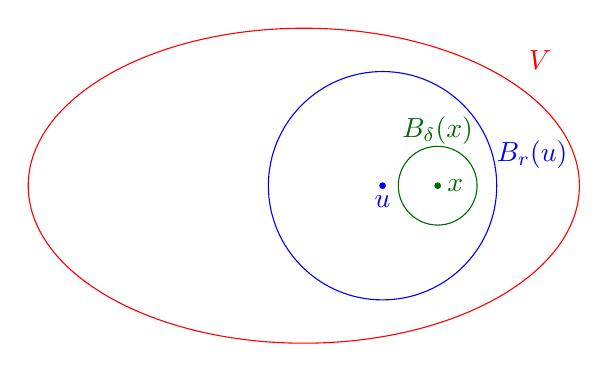
\begin{tikzpicture}
			\draw[red] (0,0) circle [x radius=3.5cm, y radius=2cm] ;
			\draw (3,1.6) node[red]{$V$};
			\draw [blue] (1,0) circle (1.45cm) ;
			\filldraw[blue] (1,0) circle (1pt) node[anchor=north]{$u$};
			\draw (2.9,0.4) node[blue]{$B_r(u)$};
			\draw [green!40!black] (1.7,0) circle (0.5cm) node [yshift=0.7cm]{$B_{\delta}(x)$} ;
			\filldraw[green!40!black] (1.7,0) circle (1pt) node[anchor=west]{$x$};
		\end{tikzpicture}
	\end{center}

	Given $x\in B_r(u)\subset V$, we want $\delta>0$ such that $x\in B_{\delta} (x)\subset B_r(u)\subset V$. Let $d=d(u,x)$. Choose $\delta $ such that $d+\delta<r$ (e.g. $\delta<\frac{r-d}{2}$)

	If $y\in B_{\delta}(x)$ we will be done by showing that $d(u,y)<r$ but $$d(u,y)\leq d(u,x)+d(x,y)<d+\delta<r$$
\end{myproof}

\cor{}{By the result of the proof, we can then show...}
\mlenma{}{Suppose $\vec{v_1}, \dots, \vec{v_n} \in \RR[n]$ is subspace of $\RR^n$.}
\mprop{}{$1 + 1 = 2$.}

\section{Random}
\dfn{Normed Linear Space and Norm $\boldsymbol{\|\cdot\|}$}{Let $V$ be a vector space over $\bbR$ (or $\bbC$). A norm on $V$ is function $\|\cdot\|\ V\to \bbR_{\geq 0}$ satisfying \begin{enumerate}[label=\bfseries\tiny\protect\circled{\small\arabic*}]
		\item \label{n:1}$\|x\|=0 \iff x=0$ $\forall$ $x\in V$
		\item \label{n:2}	$\|\lambda x\|=|\lambda|\|x\|$ $\forall$ $\lambda\in\bbR$(or $\bbC$), $x\in V$
		\item \label{n:3} $\|x+y\| \leq \|x\|+\|y\|$ $\forall$ $x,y\in V$ (Triangle Inequality/Subadditivity)
	\end{enumerate}And $V$ is called a normed linear space.

	$\bullet $ Same definition works with $V$ a vector space over $\bbC$ (again $\|\cdot\|\to\bbR_{\geq 0}$) where \ref{n:2} becomes $\|\lambda x\|=|\lambda|\|x\|$ $\forall$ $\lambda\in\bbC$, $x\in V$, where for $\lambda=a+ib$, $|\lambda|=\sqrt{a^2+b^2}$ }


\ex{$\bs{p-}$Norm}{\label{pnorm}$V={\bbR}^m$, $p\in\bbR_{\geq 0}$. Define for $x=(x_1,x_2,\cdots,x_m)\in\bbR^m$ $$\|x\|_p=\Big(|x_1|^p+|x_2|^p+\cdots+|x_m|^p\Big)^{\frac1p}$$(In school $p=2$)}
\textbf{Special Case $\bs{p=1}$}: $\|x\|_1=|x_1|+|x_2|+\cdots+|x_m|$ is clearly a norm by usual triangle inequality. \par
\textbf{Special Case $\bs{p\to\infty\ (\bbR^m$ with $\|\cdot\|_{\infty})}$}: $\|x\|_{\infty}=\max\{|x_1|,|x_2|,\cdots,|x_m|\}$\\
For $m=1$ these $p-$norms are nothing but $|x|$.
Now exercise
\qs{}{\label{exs1}Prove that triangle inequality is true if $p\geq 1$ for $p-$norms. (What goes wrong for $p<1$ ?)}
\sol{\textbf{For Property \ref{n:3} for norm-2}	\subsubsection*{\textbf{When field is $\bbR:$}} We have to show\begin{align*}
		         & \sum_i(x_i+y_i)^2\leq \left(\sqrt{\sum_ix_i^2} +\sqrt{\sum_iy_i^2}\right)^2                                       \\
		\implies & \sum_i (x_i^2+2x_iy_i+y_i^2)\leq \sum_ix_i^2+2\sqrt{\left[\sum_ix_i^2\right]\left[\sum_iy_i^2\right]}+\sum_iy_i^2 \\
		\implies & \left[\sum_ix_iy_i\right]^2\leq \left[\sum_ix_i^2\right]\left[\sum_iy_i^2\right]
	\end{align*}So in other words prove $\langle x,y\rangle^2 \leq \langle x,x\rangle\langle y,y\rangle$ where
	$$\langle x,y\rangle =\sum\limits_i x_iy_i$$

	\begin{note}
		\begin{itemize}
			\item $\|x\|^2=\langle x,x\rangle$
			\item $\langle x,y\rangle=\langle y,x\rangle$
			\item $\langle \cdot,\cdot\rangle$ is $\bbR-$linear in each slot i.e. \begin{align*}
				      \langle rx+x',y\rangle=r\langle x,y\rangle+\langle x',y\rangle	\text{ and similarly for second slot}
			      \end{align*}Here in $\langle x,y\rangle$ $x$ is in first slot and $y$ is in second slot.
		\end{itemize}
	\end{note}Now the statement is just the Cauchy-Schwartz Inequality. For proof $$\langle x,y\rangle^2\leq \langle x,x\rangle\langle y,y\rangle $$ expand everything of $\langle x-\lambda y,x-\lambda y\rangle$ which is going to give a quadratic equation in variable $\lambda $ \begin{align*}
		\langle x-\lambda y,x-\lambda y\rangle & =\langle x,x-\lambda y\rangle-\lambda\langle y,x-\lambda y\rangle                                       \\
		                                       & =\langle x ,x\rangle -\lambda\langle x,y\rangle -\lambda\langle y,x\rangle +\lambda^2\langle y,y\rangle \\
		                                       & =\langle x,x\rangle -2\lambda\langle x,y\rangle+\lambda^2\langle y,y\rangle
	\end{align*}Now unless $x=\lambda y$ we have $\langle x-\lambda y,x-\lambda y\rangle>0$ Hence the quadratic equation has no root therefore the discriminant is greater than zero.

	\subsubsection*{\textbf{When field is $\bbC:$}}Modify the definition by $$\langle x,y\rangle=\sum_i\overline{x_i}y_i$$Then we still have $\langle x,x\rangle\geq 0$}

\section{Algorithms}
\begin{algorithm}[H]
	\KwIn{This is some input}
	\KwOut{This is some output}
	\SetAlgoLined
	\SetNoFillComment
	\tcc{This is a comment}
	\vspace{3mm}
	some code here\;
	$x \leftarrow 0$\;
	$y \leftarrow 0$\;
	\uIf{$ x > 5$} {
		x is greater than 5 \tcp*{This is also a comment}
	}
	\Else {
		x is less than or equal to 5\;
	}
	\ForEach{y in 0..5} {
		$y \leftarrow y + 1$\;
	}
	\For{$y$ in $0..5$} {
		$y \leftarrow y - 1$\;
	}
	\While{$x > 5$} {
		$x \leftarrow x - 1$\;
	}
	\Return Return something here\;
	\caption{what}
\end{algorithm}

\end{document}
